\section{Auswertung}
\label{sec:Auswertung}

%\begin{figure}
%  \centering
%  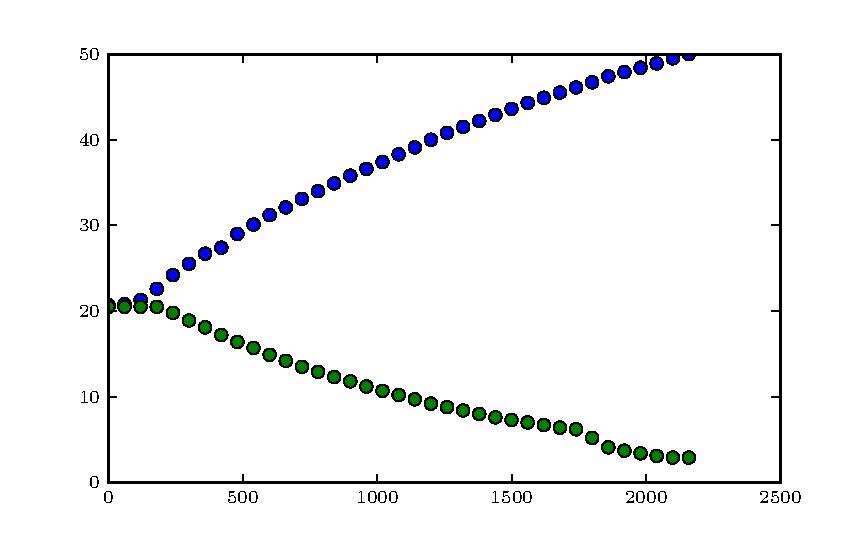
\includegraphics{plot.pdf}
%  \caption{Plot.}
%  \label{fig:plot}
%\end{figure}
\subsection{Konfiguration des Messprogramms}
\begin{figure}
  \centering
  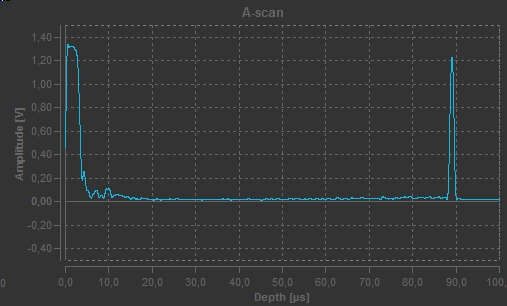
\includegraphics{Messdaten/a.jpg}
  \caption{Plot.}
  \label{fig:a1}
\end{figure}
Zur Bestimmung der Schallgeschwindigkeit im Material der vorliegenden Acrylzylinder wird die Länge eines Zylinders vermessen und die Zeitdifferenz $\Delta t$ zwischen zwei Impulsen bestimmt.
In Abbildung \ref{fig:a1} ist der Amplituden-Scan der Messung dargestellt.
Die Zeitdifferenz zwischen den beiden Maxima wird mithilfe der Cursor bestimmt zu
\begin{equation}
  \Delta t=\SI{88.69}{\micro\second} \text{.}
\end{equation}
Die Amplitudenhöhe wurde nicht vermessen, da nicht bekannt ist, wie die Verstärkung des Signals herausgerechnet werden muss.
Über die gemessene Länge des Acrylzylinders $s=\SI{120.5}{\milli\meter}$ ergibt sich mit Formel \eqref{eqn:laufzeit} eine Schallgeschwindigkeit von
\begin{equation}
  v_{\mathrm{Schall}}=\SI{2717.33}{\meter\per\second} \text{.}
\end{equation}
Da es zahlreiche unterschiedliche Literaturwerte für die Schallgeschwindigkeit in Acryl gibt, wird, dem Messergebnis folgend, für die folgende Messung eine Schallgeschwindigkeit von $v_{\mathrm{Schall}}=\SI{2720}{\meter\per\second}$ in das Messprogramm eingetragen.
Mit diesem Wert ist das Programm schließlich in der Lage, die Eindringtiefe der Schallwelle in das Material zu bestimmen.
Der Abstand zwischen den beiden Peaks entspricht dann der Länge des Acrylstabs.
Die durch das Programm berechnete Länge ergibt sich zu
\begin{equation}
  s=\SI{119.726}{\milli\meter} \text{.}
\end{equation}
\FloatBarrier

\subsection{Schallgeschwindigkeit über Impuls-Echo-Verfahren}
Die Zylinderlängen $s$ der mittels Impuls-Echo-Verfahrens vermessenen Zylinder samt der zugehörigen gemessenen Laufzeiten $t$ findet sich in Tabelle \ref{tab:iev}. In Abbildung \ref{fig:iev} sind die Zylinderlängen gegen die Laufzeiten aufgetragen. Nach Formel \eqref{eqn:laufzeit} besteht ein linearer Zusammenhang zwischen der Zylinderlänge und der Laufzeit.
Mit python/scipy \cite{scipy} wird daher eine lineare Ausgleichsrechnung nach
\begin{equation}
  y=m\cdot x +b
\end{equation}
durchgeführt.
Aus dem doppelten Steigungsparameter $m$ ergibt sich die Schallgeschwindigkeit $c_\mathrm{IE}$.
\begin{gather*}
2 \cdot m=c_\mathrm{IE}=  \SI{2738(11)}{\meter\per\second} \text{,}
b=  \SI{11(3)}{\micro\meter} \text{.}
\end{gather*}
Der Geradenparameter $b$ ist von Null verschieden, da eine Anpassungsschicht zwischen der Sonde und dem Zylinder vorliegt. Die Ausgleichsgrade ist daher nach rechts verschoben. Die Dicke der Anpassungsschicht entspricht dabei dem Geradenparameter $b$.
\begin{table}
  \centering
  \caption{bla}
  \label{tab:iev}
  \begin{tabular}{cc}
    \toprule
    s & t \\
    \midrule
    102.7 & 76.12 \\
    80.7 & 59.4 \\
    61.5 & 45.81 \\
    40.15 & 30.2 \\
    31.1 & 23.43 \\
    71.25 & 52.88 \\
    82.6 & 69.02 \\
    120.5 & 88.69 \\
    \bottomrule
  \end{tabular}
\end{table}

\begin{figure}
  \centering
  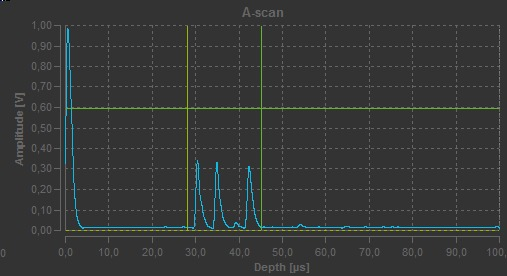
\includegraphics{Messdaten/ascan.pdf}
  \caption{Plot.}
  \label{fig:iev}
\end{figure}
\FloatBarrier

\subsection{Schallgeschwindigkeit mit dem Durchschallungsverfahren}
Die Schallgeschwindigkeit wird mittels des Durschallungsverfahren erneut bestimmt.
In Tabelle \ref{tab:durchschall} finden sich die Längen der vermessenen Zylinder sowie die zugehörigen gemessenen Laufzeiten.
In Abbildung \ref{fig:durchschall} sind die Längen der Zylinder $s$ gegen die zugehörigen Laufzeiten $t$ geplottet. Mittels python/scipy \cite{scipy} wird eine lineare Ausgleichsrechnung durchgeführt.
Nach Formel \eqref{eqn:laufzeit} ergibt sich die Schallgeschwindigkeit der Durchschallmessung $c_\mathrm{DS}$ aus dem doppelten Steigungsparameter $m$ zu:
\begin{gather*}
  2\cdot m=c_\mathrm{DS}=  \SI{2770(40)}{\meter\per\second}
  b= \SI{-53(11)}{\micro\meter}
\end{gather*}
Der Geradenparameter $b$ ist von null verschieden. Dies entsteht durch die Dicke der Anpassungsschicht beider Sonden.
\begin{figure}
  \centering
  \includegraphics{Messdaten/d.pdf}
  \caption{Plot.}
  \label{fig:durchschall}
\end{figure}
\begin{table}
  \centering
  \caption{bla}
  \label{tab:durchschall}
\begin{tabular}{cc}
  \toprule
s & t \\
\midrule
61.5 & 24.62 \\
40.15 & 16.3 \\
39.7 & 15.91 \\
31.1 & 13.31 \\
102.7 & 38.98 \\
80.7 & 30.72 \\
\bottomrule
\end{tabular}
\end{table}
\FloatBarrier
\subsection{Bestimmung der Dämpfung mit dem Impuls-Echo-Verfahren}
Über das Impuls-Echo-Verfahren wird zudem die Dämpfungskonstante des Acryls bestimmt.
Es lässt sich Formel \eqref{eqn:dampf} umformen zu:
\begin{equation}
  \ln{\left( \frac{I(x)}{I_0}\right)}=-\alpha x \text{.}
\end{equation}
Es besteht daher ein lineares Verhältnis zwischen der Dämpfungskonstante und dem Logarithmus des Amplitudenverhältnis.
In Tabelle \ref{tab:daempf} finden sich in die verwendeten Messdaten und in Abbildung \ref{fig:daempf} ist der Logarithmus des Amplitudenverhältnis aufgetragen gegen die Länge der Acrylstäbe aufgetragen.
Mittels einer linearer Ausgleichsrechnung mit python/scipy \cite{scipy} ergibt sich die Dämpfungskonstante aus der Steigung der Ausgleichsgrade:
\begin{gather*}
-m=\alpha=\SI{47(2)}{\per\meter} \text{,}
b=  \num{0.28(14)}\text{.}
\end{gather*}


\begin{table}
\centering
\caption{bla}
\label{tab:daempf}
\begin{tabular}{cccc}
  \toprule
s & a1 & a2 & ln(a1/a2) \\
\midrule
80.7 & 0.986 & 0.018 & 4.00328459671 \\
80.5 & 0.987 & 0.019 & 3.95023106027 \\
61.5 & 0.987 & 0.035 & 3.33932197794 \\
40.15 & 0.987 & 0.114 & 2.15847159104 \\
31.1 & 0.985 & 0.189 & 1.65089462611 \\
39.7 & 0.986 & 0.117 & 2.1314824198 \\
\bottomrule
\end{tabular}
\end{table}

\begin{figure}
  \centering
  \includegraphics{Messdaten/amplitude.pdf}
  \caption{Plot.}
  \label{fig:daempf}
\end{figure}
\FloatBarrier

%%%%%%%%%%%%%%%
\subsection{Auge}

Abstand Hornhaut Anfang Linse:  $\SI{6,2604}{\milli\meter}$
Avstand Hornhaut Ende Linse=  $\SI{16,0979}{\milli\meter}$
Abstand Hornhaut Retina=  $\SI{21,329}{\milli\meter}$
